% vim:ft=tex:
%
\documentclass[12pt]{article}
\usepackage{amsmath,amsfonts,amsthm}
\usepackage{graphicx}
\usepackage[top=2cm,left=1.5cm,right=1.5cm,bottom=2cm]{geometry}
\usepackage{longtable}

\title{
	JuliaSmoothOptimizers \\ SolverBenchmark.jl
}
\author{
	Abel Soares Siqueira \\ Dominique Orban
}
\date{ }

\begin{document}
\maketitle

\section*{Output of solver alpha}

\begin{longtable}[c]{lrrrr}
\hline 
flag & name & \(f(x)\) & time & iter \\
\hline 
\endfirsthead
\multicolumn{5}{l}
{{\bfseries \tablename\ \thetable{} --- continued from previous page}} \\
\hline 
flag & name & \(f(x)\) & time & iter \\
\hline 
\endhead
\hline 
\multicolumn{5}{r}{{\bfseries Continued on next page}} \\
\hline 
\endfoot
\hline 
\endlastfoot
failure & prob001 & \(-6.9\)e\(-01\) & \( 6.2\)e\(+01\) & \(   70\) \\
failure & prob002 & \(-7.6\)e\(-01\) & \( 3.5\)e\(+02\) & \(   10\) \\
success & prob003 & \( 4.0\)e\(-01\) & \( 7.7\)e\(+02\) & \(   10\) \\
success & prob004 & \( 8.1\)e\(-01\) & \( 4.3\)e\(+01\) & \(   80\) \\
success & prob005 & \(-3.5\)e\(-01\) & \( 2.7\)e\(+02\) & \(   30\) \\
success & prob006 & \(-1.9\)e\(-01\) & \( 6.7\)e\(+01\) & \(   80\) \\
success & prob007 & \(-1.6\)e\(+00\) & \( 1.6\)e\(+02\) & \(   60\) \\
success & prob008 & \(-2.5\)e\(+00\) & \( 6.1\)e\(+02\) & \(   40\) \\
success & prob009 & \( 2.3\)e\(+00\) & \( 1.4\)e\(+02\) & \(   40\) \\
failure & prob010 & \( 2.2\)e\(-01\) & \( 8.4\)e\(+02\) & \(   50\) \\
\hline 
\end{longtable}


\section*{Joined output}

\begin{longtable}[c]{lrrrrrrrrrr}
\hline 
id & name & flag\_alpha & f\_alpha & t\_alpha & flag\_beta & f\_beta & t\_beta & flag\_gamma & f\_gamma & t\_gamma \\
\hline 
\endfirsthead
\multicolumn{11}{l}
{{\bfseries \tablename\ \thetable{} --- continued from previous page}} \\
\hline 
id & name & flag\_alpha & f\_alpha & t\_alpha & flag\_beta & f\_beta & t\_beta & flag\_gamma & f\_gamma & t\_gamma \\
\hline 
\endhead
\hline 
\multicolumn{11}{r}{{\bfseries Continued on next page}} \\
\hline 
\endfoot
\hline 
\endlastfoot
\(    1\) & prob001 & failure & \(-6.9\)e\(-01\) & \( 6.2\)e\(+01\) & success & \(-1.1\)e\(+00\) & \( 1.8\)e\(+02\) & success & \( 6.3\)e\(-02\) & \( 3.3\)e\(+01\) \\
\(    2\) & prob002 & failure & \(-7.6\)e\(-01\) & \( 3.5\)e\(+02\) & failure & \( 8.2\)e\(-01\) & \( 8.0\)e\(+01\) & success & \( 1.2\)e\(-01\) & \( 6.9\)e\(+02\) \\
\(    3\) & prob003 & success & \( 4.0\)e\(-01\) & \( 7.7\)e\(+02\) & success & \( 1.5\)e\(-01\) & \( 6.8\)e\(+02\) & success & \( 2.7\)e\(+00\) & \( 8.4\)e\(+02\) \\
\(    4\) & prob004 & success & \( 8.1\)e\(-01\) & \( 4.3\)e\(+01\) & failure & \(-3.3\)e\(-01\) & \( 9.3\)e\(+02\) & failure & \(-6.9\)e\(-01\) & \( 1.9\)e\(+02\) \\
\(    5\) & prob005 & success & \(-3.5\)e\(-01\) & \( 2.7\)e\(+02\) & failure & \( 1.4\)e\(+00\) & \( 9.7\)e\(+02\) & failure & \(-5.5\)e\(-02\) & \( 1.6\)e\(+02\) \\
\(    6\) & prob006 & success & \(-1.9\)e\(-01\) & \( 6.7\)e\(+01\) & success & \(-4.4\)e\(-01\) & \( 6.5\)e\(+02\) & success & \( 4.2\)e\(-01\) & \( 9.0\)e\(+02\) \\
\(    7\) & prob007 & success & \(-1.6\)e\(+00\) & \( 1.6\)e\(+02\) & success & \( 1.1\)e\(+00\) & \( 6.0\)e\(+02\) & success & \(-1.4\)e\(+00\) & \( 9.5\)e\(+01\) \\
\(    8\) & prob008 & success & \(-2.5\)e\(+00\) & \( 6.1\)e\(+02\) & success & \(-2.5\)e\(-01\) & \( 4.8\)e\(+02\) & failure & \(-4.5\)e\(-01\) & \( 7.8\)e\(+02\) \\
\(    9\) & prob009 & success & \( 2.3\)e\(+00\) & \( 1.4\)e\(+02\) & failure & \( 2.9\)e\(-01\) & \( 6.3\)e\(+01\) & failure & \(-8.8\)e\(-01\) & \( 8.7\)e\(+02\) \\
\(   10\) & prob010 & failure & \( 2.2\)e\(-01\) & \( 8.4\)e\(+02\) & success & \(-3.5\)e\(+00\) & \( 4.7\)e\(+02\) & success & \( 1.1\)e\(+00\) & \( 8.4\)e\(+02\) \\
\hline 
\end{longtable}


\section*{Profiles}

\begin{center}
  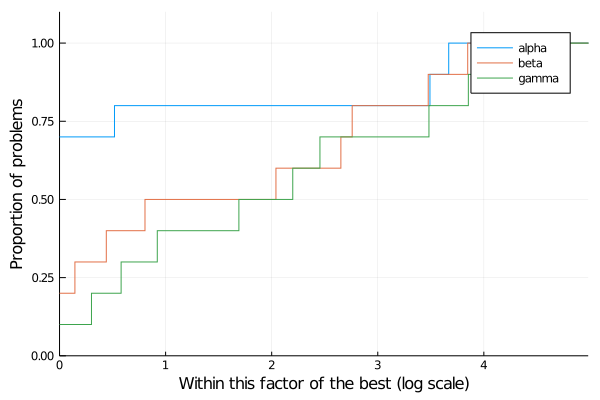
\includegraphics[width=0.66\textwidth]{profile1}

  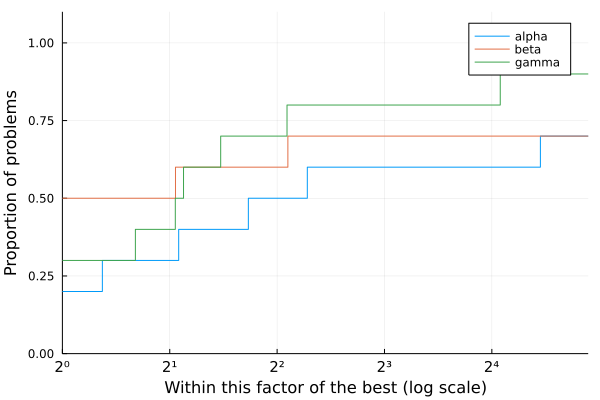
\includegraphics[width=0.66\textwidth]{profile2}
\end{center}

\end{document}
